%========================================================================================
% TU Dortmund, Informatik Lehrstuhl VII
%========================================================================================

\chapter{Einleitung}
\label{Einleitung}

\section{Motivation und Hintergrund}
\label{Motivation_und_Hintergrund}
%
Das Höchstspannungsnetz, welches sich über Deutschland erstreckt ist riesig und besteht aus tausenden von Strommasten und Verbindungen. Da ist sehr vom Nutzen eine Karte zu haben, die einige Verbindungen und Orte verschiebt um eine weitaus bessere und übersichtlichere Darstellung zu erhalten. Das ist genau die Methode einer MetroMap, den Verlust genauer Daten um sicherzustellen, dass die wichtigen Verbindungen und Standorte schnell und sicher erkannt werden.
\\
In dieser Arbeit geht es darum, die Methoden einer MetroMap für Bus- und Bahnverbindungen zu nutzen, um eine angepasste MetroMap für das deutsche Höchstspannungsnetz zu erhalten. 


    \begin{figure}[t]
    	\centering
    	{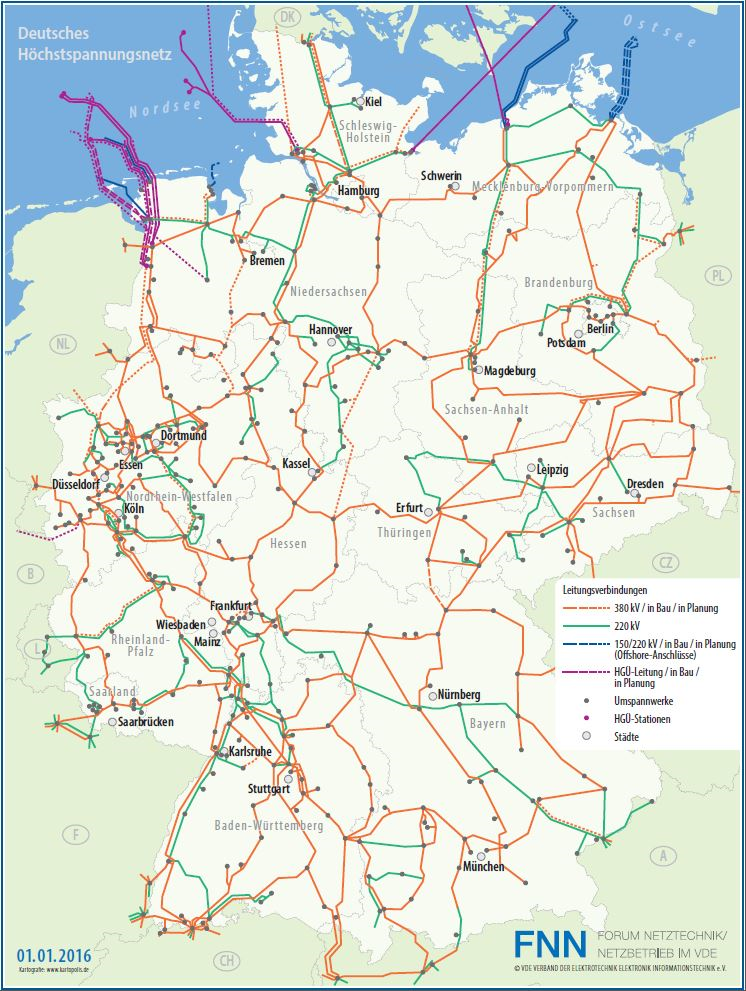
\includegraphics[scale=0.5]{bilder/hochstspannungsnetz}\label{fig_hochstspannungsnetz}
    	}\\
    	\caption[Karte des deutschen Höchstspannungsnetzes]{Karte des deutschen Höchstspannungsnetzes}
    	\label{fig_hochstspannungsnetz2}
    \end{figure}
        \begin{figure}[t]
        	\centering
        	{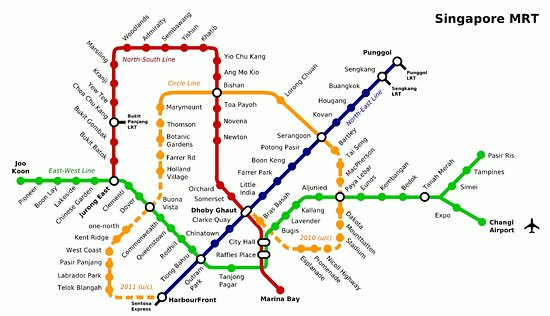
\includegraphics[scale=0.5]{bilder/metromapsinga}\label{fig_metromapsinga}
        	}\\
        	\caption[MetroMap der Bahnverbindungen in Singapur]{MetroMap der Bahnverbindungen in Singapur}
        	\label{fig_metromapsinga2}
        \end{figure}

\section{Aufbau der Arbeit}
\label{Aufbau_der_Arbeit}
%

